\section{Worksheet 7}
\begin{lstlisting}
bool PointLight::emit(Ray& r, HitInfo& hit, float3& Phi) const
{
	float3 direction;
	do{
		direction.x = 2.0f * mt_random() - 1.0f;
		direction.y = 2.0f * mt_random() - 1.0f;
		direction.z = 2.0f * mt_random() - 1.0f;
	}while (dot(direction, direction) > 1.0f);
	direction = normalize(direction);
	r = Ray(light_pos, direction, 1,1e-4, RT_DEFAULT_MAX);
	
	// Trace ray
	tracer->trace_to_closest(r, hit);
	
	// If a surface was hit, compute Phi and return true
	if (hit.has_hit) {
		Phi = intensity*4*M_PIf;
	}
	return hit.has_hit;
}

void ParticleTracer::trace_particle(const Light* light, const unsigned int caustics_done)
{
	if(caustics_done)
		return;
	
	// Shoot a particle from the sampled source
	Ray r;
	HitInfo hit;
	float3 Phi;
	if (!light->emit(r, hit, Phi)|| !scene->is_specular(hit.material)) {
		return;
	}
	
	// Forward from all specular surfaces
	while(scene->is_specular(hit.material) && hit.trace_depth < 500){
		switch(hit.material->illum)
		{
		case 3:  // mirror materials
			{
				// Forward from mirror surfaces here
				return;
			}
			break;
		case 11: // absorbing volume
		case 12: // absorbing glossy volume
			{
				// Handle absorption here (Worksheet 8)
			}
		case 2:  // glossy materials
		case 4:  // transparent materials
			{
				Ray refracted;
				HitInfo hit_refracted;
				float probability;
				
				trace_refracted(r, hit, refracted, hit_refracted, probability);
				
				float epsilon = mt_random();
				if (epsilon < probability) {
					Ray reflected;
					HitInfo hit_reflected;
					trace_reflected(r, hit, reflected, hit_reflected);
					r = reflected;
					hit = hit_reflected;
				}
				else {
					r = refracted;
					hit = hit_refracted;
				}
				if (!hit.has_hit) {
					return;
				}
			}
			break;
		default: 
			return;
		}
	}
	caustics.store(Phi,hit.position,-r.direction);
}
\end{lstlisting}

\begin{figure}[H]
	\centering
	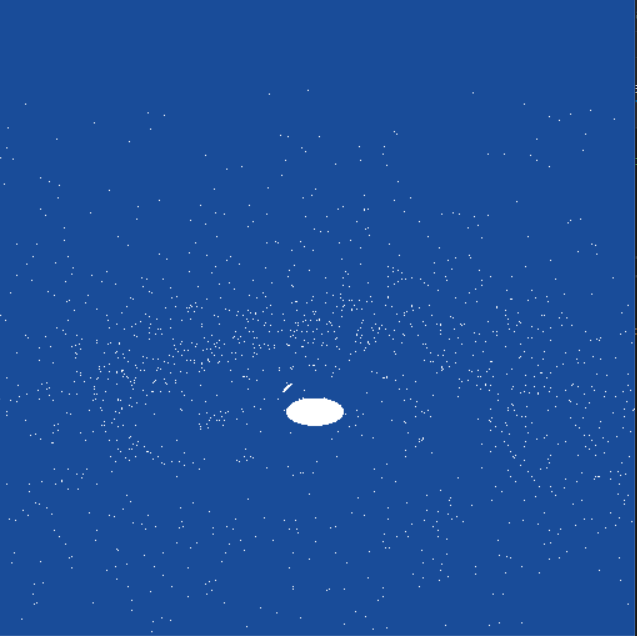
\includegraphics[scale=\imagescale]{images/worksheet_7/caustics_preview}
	\caption{Caustics preview}
	\label{fig:caustics_preview}
\end{figure}

\begin{lstlisting}
float3 PhotonCaustics::shade(const Ray& r, HitInfo& hit, bool emit) const
{	
	float3 irradiance=tracer->caustics_irradiance(hit,max_dist,photons);
	float3 radiance = irradiance * rho_d / M_PIf;
	return Lambertian::shade(r, hit, emit)+ radiance;
}
\end{lstlisting}

\begin{figure}[H]
	\centering
	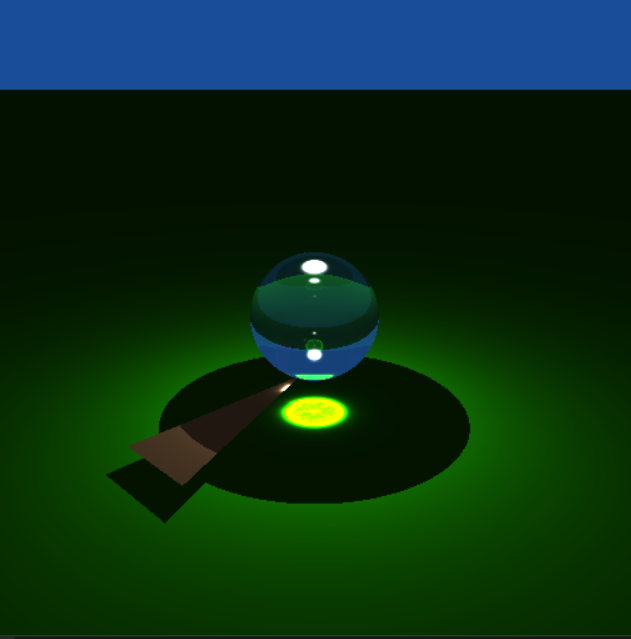
\includegraphics[scale=\imagescale]{images/worksheet_7/caustics_full_illum}
	\caption{Caustics and full illumination}
	\label{fig:caustics_full_illum}
\end{figure}

\begin{figure}[H]
	\centering
	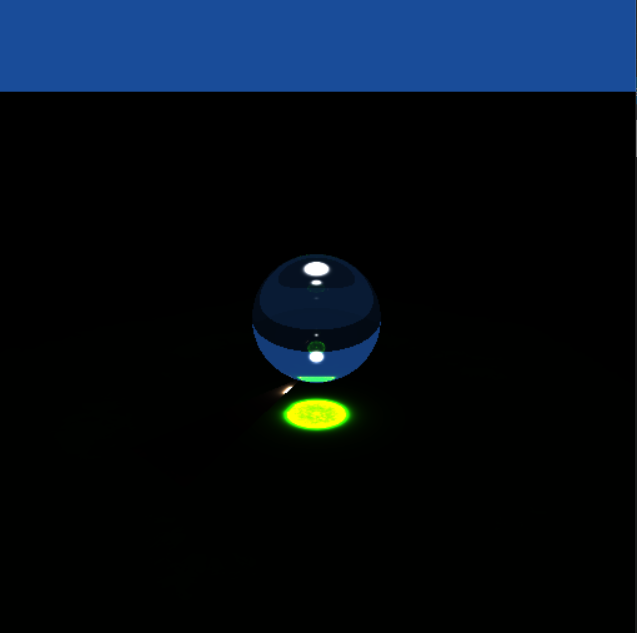
\includegraphics[scale=\imagescale]{images/worksheet_7/caustics_only}
	\caption{Caustics illumination only}
	\label{fig:caustics_only}
\end{figure}
